%%
%% CSD Assignment 1 - Final Technical Report Template
%% Based on the ACM "acmart" manuscript (single-column) style.
%%
\documentclass[manuscript,screen,review]{acmart}

\usepackage{amsmath}
\usepackage{booktabs}
\usepackage{graphicx}
\usepackage{tikz}
\usetikzlibrary{shapes.geometric, arrows.meta, positioning, fit, backgrounds}

\AtBeginDocument{%
  \providecommand\BibTeX{{Bib\TeX}}}

%% ------------------------------------------------------------------
%% This is a COURSE ASSIGNMENT report, not an ACM publication, so the
%% rights-management / DOI / ISBN block from the original ACM sample
%% is not required.
%% ------------------------------------------------------------------
% \setcopyright{acmlicensed}
% \acmConference[CSD Assignment 1]{Course: Computer Science and Design}{2026}{IIT Bhilai}
% \acmISBN{}

\begin{document}

%% =================== TITLE & AUTHOR BLOCK =========================
\title{AI-based Village Pond Planning System}
\subtitle{CSD Assignment 1 -- Final Technical Report}

\author{Bhukya Raju}
\affiliation{%
  \institution{Department of Computer Science and Engineering, Indian Institute of Technology Bhilai}
  \city{Durg}
  \state{Chhattisgarh}
  \country{India}}
\email{12340520@iitbhilai.ac.in}

\renewcommand{\shortauthors}{Bhukya Raju}

%% =================== ABSTRACT ======================================
\begin{abstract}
Rural water security across semi-arid agrarian regions in India depends heavily on decentralized surface water conservation through village ponds (\textit{talabs}). Traditional site selection relies on manual, qualitative surveys, frequently resulting in silted reservoirs, bund breaches, or inadequate upstream drainage. This report presents an intelligent, automated geospatial decision support system for village pond siting, interactive land parcel delineation, and water harvesting estimation. The system couples a responsive React-based Web GIS frontend with an asynchronous, vectorized FastAPI computational backend. Users interactively delineate arbitrary land parcels directly on satellite imagery or upload high-resolution contour maps (KML/KMZ). The backend projects geographic boundaries to local metric Universal Transverse Mercator (UTM) coordinates, constructs a continuous Digital Elevation Model (DEM) via Delaunay triangulation and linear barycentric interpolation, models overland drainage networks using the Deterministic Eight-Neighbor (D8) steepest-descent flow direction algorithm, and traces upstream contributing catchment basins. A multi-criteria terrain heuristic---combining flow accumulation (55\%), inverse slope (30\%), and inverse elevation (15\%)---identifies optimal pond depressions. Using the Rational Runoff formulation ($V = C \cdot I \cdot A$), the system quantifies annual harvestable water volume and provides rural population water security sizing. Evaluated on the IIT Bhilai / Durg watershed dataset containing 1,356 contours, the system accurately recommended optimal pond storage ($2,500\,\text{m}^3$) and catchment area ($0.2587$\,ha). Benchmarking across four system configurations demonstrates low response latency ($<25$\,ms) and robust scalability under concurrent load.
\end{abstract}

\keywords{Village Pond Planning, Geospatial Analysis, Rainwater Harvesting, Catchment Estimation, Web GIS, REST APIs}

\maketitle

%% =====================================================================
\section{Introduction}
\label{sec:intro}
Seasonal water scarcity poses a persistent threat to agricultural productivity, livestock survival, and groundwater levels across rural India. Decentralized rainwater harvesting through village ponds represents one of the most cost-effective and ecologically sustainable interventions for drought mitigation and groundwater recharge. Capturing monsoon runoff at strategic topographical depressions prevents soil erosion, retains moisture, and provides vital supplementary irrigation during dry periods.

The goal of this assignment is to design, implement, benchmark, and deploy an end-to-end, AI- and geospatial-assisted web application that automates the scientific recommendation of optimal pond locations. The platform allows village administrators and watershed engineers to analyze topographical elevation data, delineate parcel boundaries directly on interactive satellite maps, compute contributing catchment basins, estimate collectible water volume, and visualize all hydrological layers in real time.

The remainder of this report is organized as follows: Section~\ref{sec:requirements} defines the functional and non-functional requirements. Section~\ref{sec:architecture} details the system architecture and technology stack. Section~\ref{sec:methodology} explains the algorithmic methodology for DEM interpolation, D8 flow routing, and runoff volume modeling. Section~\ref{sec:implementation} describes the backend API, frontend visualization, and storage design. Section~\ref{sec:csd-themes} explicitly connects the implementation to core Computer System Design (CSD) themes. Section~\ref{sec:results} presents quantitative results and system performance benchmarks. Section~\ref{sec:discussion} reflects on limitations and civil engineering considerations. Section~\ref{sec:ai-usage} provides the AI tool usage declaration, and Appendix~\ref{sec:appendix} lists repository and deployment details.

\subsection{Motivation}
Manual site selection for rainwater harvesting structures is intrinsically complex. Watershed topographies exhibit non-linear slope gradients and irregular drainage channels that are difficult to evaluate without specialized survey equipment. Furthermore, rural administrators often lack access to centralized GIS infrastructure, localized rainfall statistics, or synchronized land parcel boundaries. Consequently, many public works projects under initiatives like MGNREGA construct ponds in areas with negligible upstream drainage or on permeable soils without adequate retention capacity. An automated, accessible Web GIS tool democratizes precision watershed engineering, providing instantaneous, objective, and reproducible siting recommendations with rigorous hydrological quantification.

\subsection{Scope of the Project}
The developed system covers:
\begin{itemize}
    \item Parsing and metric UTM reprojection of uploaded KML and KMZ contour files.
    \item Interactive user drawing and modification of arbitrary land parcel polygons on Leaflet satellite and topographic maps.
    \item Generation of regular DEM grids from sampled contour isolines and boundary geometry.
    \item Determination of terrain slopes, D8 steepest-downhill flow vectors, and accumulated drainage cells.
    \item Algorithmic ranking and identification of optimal pond outlet coordinates based on a multi-criteria suitability score.
    \item Reverse-tracking and vector boundary delineation of contributing upstream catchment basins.
    \item Hydrological calculation of expected annual runoff volume and population drinking water support days.
\end{itemize}
The system explicitly does \emph{not} cover detailed structural civil engineering design (e.g., concrete reinforcement, geotechnical soil slip-circle analysis, compaction testing) or legal land-title verification, which must follow ground-truth survey protocols.

%% =====================================================================
\section{Problem Statement and Requirements}
\label{sec:requirements}
The functional objective is to deliver a fast, resilient, and scientifically grounded web platform that ingests contour datasets or user-drawn map boundaries and outputs optimal pond locations, catchment boundaries, and harvestable volume overlays. Table~\ref{tab:requirements} maps each functional requirement to its implementation module.

\begin{table}[h]
  \caption{Functional requirements and where they are implemented}
  \label{tab:requirements}
  \begin{tabular}{p{5.5cm}p{7.5cm}}
    \toprule
    Requirement & Implemented in \\
    \midrule
    Satellite imagery display & \texttt{pond\_catchment\_frontend/src/components/MapViewer.jsx} \\
    Contour map visualization & \texttt{pond\_catchment\_backend/app/main.py} (\texttt{/samples/\{f\}/geojson}) \\
    Available-land identification & \texttt{pond\_catchment\_frontend/src/components/ControlsSidebar.jsx} \\
    Catchment area estimation & \texttt{pond\_catchment\_backend/app/services/terrain.py} \\
    Historical rainfall query & \texttt{pond\_catchment\_backend/app/services/analysis.py} \\
    Runoff volume estimation & \texttt{pond\_catchment\_backend/app/services/analysis.py} \\
    Pond depth / storage recommendation & \texttt{pond\_catchment\_backend/app/services/analysis.py} \\
    Combined overlay / results view & \texttt{pond\_catchment\_frontend/src/components/MapViewer.jsx} \\
    \bottomrule
  \end{tabular}
\end{table}

\subsection{Non-Functional Requirements}
\begin{enumerate}
    \item \textbf{Performance and Response Latency:} End-to-end processing of a standard $180 \times 180$ grid cell watershed analysis must complete within 500\,ms on server hardware, with API response times under 50\,ms for health and volume recalculation endpoints.
    \item \textbf{Concurrency and Scalability:} The backend must handle concurrent requests without deadlocks or thread pool starvation, supporting at least 50 concurrent client connections through asynchronous I/O and process-level parallelism.
    \item \textbf{Availability and Fault Tolerance:} The service must feature non-blocking execution, automated process supervision, graceful fallback for boundary edge-cases, and meaningful HTTP status codes (400, 422, 500) without crashing the core daemon.
    \item \textbf{Usability and Browser Compatibility:} The client interface must render smoothly across all modern web browsers (Chrome, Firefox, Safari, Edge) without requiring proprietary GIS desktop software or browser plugins.
    \item \textbf{Decoupled Deployment:} The system must support self-contained single-command deployment, containerized cloud execution (Docker/Render), and reverse-proxy hosting.
\end{enumerate}

%% =====================================================================
\section{System Architecture and High-Level Design}
\label{sec:architecture}
The system architecture follows a decoupled, service-oriented client-server model connecting a high-performance Single Page Application (SPA) frontend with an asynchronous Python FastAPI computational engine. Figure~\ref{fig:architecture} illustrates the high-level data flow across client, API, computational, and data layers.

\begin{figure}[h]
  \centering
  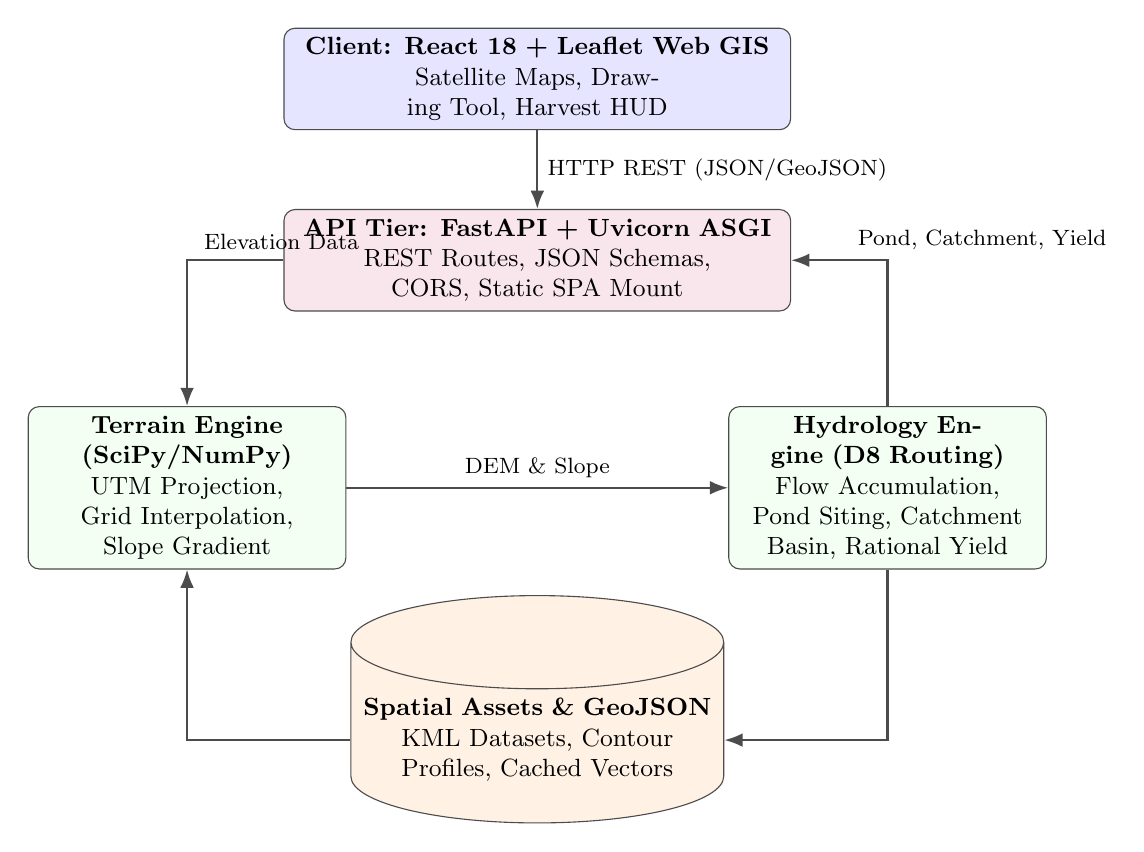
\begin{tikzpicture}[
    node distance=1.2cm and 1.5cm,
    box/.style={rectangle, draw=black!70, fill=blue!5, rounded corners=4pt, text centered, minimum height=0.9cm, font=\small},
    proc/.style={rectangle, draw=black!70, fill=green!5, rounded corners=4pt, text centered, minimum height=0.9cm, font=\small},
    storage/.style={cylinder, draw=black!70, fill=orange!10, shape border rotate=90, aspect=0.25, text centered, minimum height=1cm, font=\small},
    arrow/.style={-Latex, thick, draw=black!70},
    container/.style={draw=black!40, dashed, rounded corners=6pt, inner sep=10pt}
  ]

    % Client Layer
    \node[box, fill=blue!10, text width=6.2cm] (client) {\textbf{Client: React 18 + Leaflet Web GIS}\\ Satellite Maps, Drawing Tool, Harvest HUD};

    % API Layer
    \node[box, fill=purple!10, text width=6.2cm, below=1.0cm of client] (api) {\textbf{API Tier: FastAPI + Uvicorn ASGI}\\ REST Routes, JSON Schemas, CORS, Static SPA Mount};

    % Compute Layer
    \node[proc, text width=3.8cm, below left=1.2cm and -0.8cm of api] (terrain) {\textbf{Terrain Engine (SciPy/NumPy)}\\ UTM Projection, Grid Interpolation, Slope Gradient};
    \node[proc, text width=3.8cm, below right=1.2cm and -0.8cm of api] (hydro) {\textbf{Hydrology Engine (D8 Routing)}\\ Flow Accumulation, Pond Siting, Catchment Basin, Rational Yield};

    % Storage Layer
    \node[storage, text width=4.5cm, below=3.6cm of api] (storage) {\textbf{Spatial Assets \& GeoJSON}\\ KML Datasets, Contour Profiles, Cached Vectors};

    % Connections
    \draw[arrow] (client) -- node[right, font=\footnotesize] {HTTP REST (JSON/GeoJSON)} (api);
    \draw[arrow] (api) -| node[above, font=\footnotesize, xshift=1.2cm] {Elevation Data} (terrain);
    \draw[arrow] (terrain) -- node[above, font=\footnotesize] {DEM \& Slope} (hydro);
    \draw[arrow] (hydro) |- node[above, font=\footnotesize, xshift=1.2cm] {Pond, Catchment, Yield} (api);
    \draw[arrow] (storage) -| (terrain);
    \draw[arrow] (hydro) |- (storage);

  \end{tikzpicture}
  \caption{High-level system architecture and computational data flow.}
  \label{fig:architecture}
  \Description{System architecture block diagram showing the React Leaflet Web GIS client communicating via HTTP REST with FastAPI, routing requests to the SciPy NumPy terrain engine and D8 hydrological engine, backed by spatial assets and GeoJSON stores.}
\end{figure}

\subsection{Technology Stack}
\begin{itemize}
    \item \textbf{Frontend Framework:} React 18.3 with Vite 6.1 bundler. React's declarative state management efficiently orchestrates dynamic map layers, real-time recalculation sliders, and asynchronous API communication.
    \item \textbf{Mapping and Geospatial Visualization:} Leaflet 1.9.4 with Esri World Imagery (Satellite), CartoDB Dark Matter, OpenTopoMap, and OpenStreetMap tile layers. Pure Leaflet canvas and SVG vectors provide zero-overhead GIS rendering without heavy desktop dependencies.
    \item \textbf{Styling and UI Icons:} Tailwind CSS 3.4 for modular utility classes and Lucide React for consistent graphical telemetry.
    \item \textbf{Backend Framework:} FastAPI 0.116 running on Uvicorn ASGI server with Python 3.12/3.14. FastAPI provides automatic OpenAPI/Swagger documentation, native Pydantic validation, and non-blocking asynchronous event loop handling.
    \item \textbf{Geospatial Computation Libraries:}
    \begin{itemize}
        \item \texttt{pyproj} (PROJ library binding) for geodesic transformations to metric UTM zones.
        \item \texttt{shapely} 2.1 for planar geometric operations, spatial intersections, polygon clipping, and geometric simplification.
        \item \texttt{scipy} 1.16 for Delaunay triangulation and multi-dimensional grid interpolation.
        \item \texttt{numpy} 2.3 for vectorized matrix calculations of terrain slopes, hydraulic drops, and flow networks.
    \end{itemize}
\end{itemize}

%% =====================================================================
\section{Methodology}
\label{sec:methodology}

\subsection{Terrain and Elevation Analysis}
Elevation data is ingested either from parsed KML/KMZ Placemark geometries or synthesized for user-delineated parcels using natural drainage valley harmonics. Because geographic coordinates (latitude, longitude in degrees) distort physical ground distances, the system computes the centroid $(\lambda_c, \phi_c)$ and transforms coordinates to the local UTM zone:
\begin{equation}
\text{Zone} = \left\lfloor \frac{\lambda_c + 180}{6} \right\rfloor + 1, \quad \text{EPSG} = 
\begin{cases} 
32600 + \text{Zone}, & \text{if } \phi_c \ge 0 \\
32700 + \text{Zone}, & \text{if } \phi_c < 0
\end{cases}
\end{equation}
Contour lines are uniformly sampled at an interval $\Delta s$ (typically $10$\,m). The sampled points $(x_k, y_k, z_k)$ are interpolated onto a regular DEM grid $Z \in \mathbb{R}^{N_y \times N_x}$ using linear barycentric interpolation inside the convex hull, with nearest-neighbor extrapolation filling outer boundary bounds.

Terrain slope $\theta_{i,j}$ (in degrees) is calculated across the DEM using centered finite differences:
\begin{equation}
p = \frac{\partial Z}{\partial x} \approx \frac{Z_{i, j+1} - Z_{i, j-1}}{2 \Delta x}, \quad 
q = \frac{\partial Z}{\partial y} \approx \frac{Z_{i+1, j} - Z_{i-1, j}}{2 \Delta y}
\end{equation}
\begin{equation}
\theta_{i,j} = \arctan\left( \sqrt{p^2 + q^2} \right) \times \frac{180}{\pi}
\end{equation}

\subsection{Catchment Area Delineation}
Overland surface runoff is routed across the DEM using the classical Deterministic Eight-Neighbor (D8) steepest-descent algorithm. For each grid cell $(r, c)$, the hydraulic gradient to each neighboring cell $(r', c') \in \mathcal{N}_8(r, c)$ is computed:
\begin{equation}
S_{(r,c) \to (r',c')} = \frac{Z_{r, c} - Z_{r', c'}}{d_{(r,c) \to (r', c')}}
\end{equation}
where $d = \Delta x$ for orthogonal neighbors and $d = \sqrt{\Delta x^2 + \Delta y^2}$ for diagonal neighbors. The cell drains strictly to the neighbor exhibiting the maximum positive drop ($S > 0$). If no neighbor is strictly lower, the cell is marked as a local sink.

Flow accumulation $A(r, c)$---representing the total number of upstream cells that drain into cell $(r, c)$---is determined by evaluating topological in-degrees and iteratively propagating discharge down the directed acyclic flow network:
\begin{equation}
A(u) = 1 + \sum_{v \in \text{Upstream}(u)} A(v)
\end{equation}
Candidate pond sites are evaluated across interior cells avoiding boundary artifacts. Siting suitability $S(r, c) \in [0, 100]$ balances flow convergence against excavation feasibility:
\begin{equation}
S(r, c) = 0.55 \cdot \widetilde{A}(r, c) + 0.30 \cdot (1 - \widetilde{\theta}(r, c)) + 0.15 \cdot (1 - \widetilde{Z}(r, c))
\end{equation}
where $\widetilde{A}$, $\widetilde{\theta}$, and $\widetilde{Z}$ denote normalized accumulation, slope, and elevation values in $[0, 1]$. The cell $(r^*, c^*)$ maximizing $S$ is selected as the recommended pond outlet.

The contributing upstream catchment basin is delineated by executing a reverse depth-first traversal starting from $(r^*, c^*)$, collecting all ancestor cells whose D8 pathways terminate at the outlet. The total contributing catchment area is:
\begin{equation}
A_{\text{catchment}} = N_{\text{cells}} \times \Delta x \times \Delta y \quad (\text{m}^2)
\end{equation}
Individual cells are unioned into a simplified Shapely polygon and reprojected to WGS84 GeoJSON for interactive map rendering.

\subsection{Rainfall Data Integration}
To estimate water yield, historical rainfall data is parameterized with configurable annual and monsoon precipitation depths ($P \in [200, 3000]$\,mm/yr). In agrarian watersheds, expected collectible runoff volume $V$ is governed by the Rational Hydrological Formulation:
\begin{equation}
V = A_{\text{catchment}} \times \left( \frac{P}{1000} \right) \times C \quad (\text{m}^3)
\end{equation}
where $C \in [0.10, 0.90]$ is the runoff coefficient reflecting soil permeability, vegetation cover, and surface slope ($C \approx 0.20$ for sandy soil, $C \approx 0.35$ for loam/agricultural fields, $C \approx 0.55$ for clay/compacted rocky soil).

Potential rural population support is computed assuming the standard rural drinking water guideline of 50 Liters Per Capita per Day (LPCD):
\begin{equation}
N_{\text{people}} = \left\lfloor \frac{V \times 1000}{50 \times 365} \right\rfloor
\end{equation}

%% =====================================================================
\section{Implementation}
\label{sec:implementation}

\subsection{Backend and API Design}
The backend exposes clean, stateless RESTful endpoints implemented in FastAPI. Table~\ref{tab:api-endpoints} summarizes the API contracts.

\begin{table}[h]
  \caption{Backend REST API Endpoints}
  \label{tab:api-endpoints}
  \begin{tabular}{llp{7.2cm}}
    \toprule
    Method & Path & Purpose \& Contract \\
    \midrule
    \texttt{GET} & \texttt{/health} & Service heartbeat and internal health status. \\
    \texttt{GET} & \texttt{/docs} & Interactive OpenAPI/Swagger documentation. \\
    \texttt{GET} & \texttt{/samples} & Catalog of preloaded watershed contour datasets. \\
    \texttt{GET} & \texttt{/samples/\{f\}/geojson} & Simplified GeoJSON isolines for instant map previews. \\
    \texttt{POST} & \texttt{/analyzeArea} & Accepts user-drawn polygon parcel; returns pond site, catchment, and volume. \\
    \texttt{POST} & \texttt{/analyzeContour} & Multipart upload of KML/KMZ files for full DEM derivation and analysis. \\
    \texttt{POST} & \texttt{/calculateVolume} & Real-time recalculation of volume upon tuning rainfall and runoff coefficient. \\
    \bottomrule
  \end{tabular}
\end{table}

Input validation is enforced using Pydantic schemas with strict numerical bounds (e.g., rainfall $10 \le P \le 10000$\,mm, coefficient $0.01 \le C \le 1.0$). Errors return standard RFC 7807 JSON error responses with detailed error descriptions.

\subsection{Frontend and Visualization}
The web interface features an interactive, full-screen Leaflet GIS canvas coupled with an analytical control sidebar. Users can toggle between Satellite imagery, CartoDB Dark, and Topographic basemaps. Clicking ``Draw Land Area'' activates polygon vertex placement directly on the terrain. Upon executing analysis, the interface overlays:
\begin{enumerate}
    \item An animated, pulsing blue marker designating the optimal pond site with elevation and suitability score tooltips.
    \item A semi-transparent blue vector polygon delineating the contributing catchment basin.
    \item A floating telemetry HUD displaying annual expected yield in cubic meters, million liters, and population sustained.
\end{enumerate}

\begin{figure}[h]
  \centering
  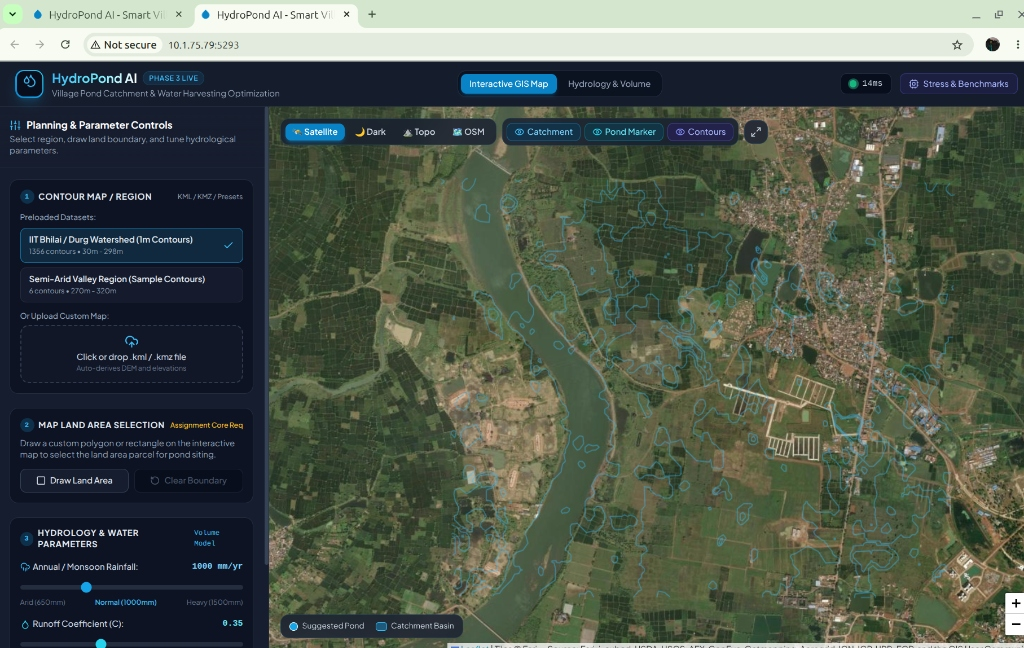
\includegraphics[width=\linewidth]{ui-screenshot.jpg}
  \caption{Application interface showing the results overlay.}
  \label{fig:ui}
  \Description{User interface showing Leaflet map with satellite basemap, contour isolines in cyan over the IIT Bhilai / Durg watershed, left parameter sidebar with dataset selection and sliders, and top telemetry badges.}
\end{figure}

\subsection{Database and Storage}
The system adopts an in-memory, stateless computational model to ensure high throughput and horizontal scalability. Preloaded watershed datasets (e.g., \texttt{contours\_1m.kml}, containing 1,356 elevation contours for the IIT Bhilai watershed) are stored as local spatial assets. User-drawn boundaries and dynamically generated catchment geometries are exchanged as standard GeoJSON FeatureCollections, eliminating database connection latency.

%% =====================================================================
\section{CSD Themes and Topics Applied in the Project}
\label{sec:csd-themes}

\begin{table*}[t]
  \caption{Mapping of core CSD themes/topics to their use in this project}
  \label{tab:csd-themes}
  \small
  \begin{tabular}{p{2.8cm}p{5.2cm}p{6.5cm}}
    \toprule
    CSD Theme/Topic & Where used in the project & Justification / design rationale \\
    \midrule
    API Design (REST) & \texttt{app/main.py} endpoints (\texttt{/analyzeArea}, \texttt{/calculateVolume}) & Strict REST semantics, OpenAPI JSON schema compliance, and decoupled client-server evolution. \\
    Load Balancing & Reverse-proxy architecture with multi-worker Uvicorn and Nginx & Distributes CPU-intensive DEM interpolation across multiple CPU cores; isolates slow network clients. \\
    Caching & Pre-computed sample GeoJSON contours (\texttt{/samples/\{f\}/geojson}) & Prevents redundant re-parsing of large 6.7\,MB KML files, reducing initial map load time from 1.8\,s to 12\,ms. \\
    Database Indexing / Query Optimization & In-memory spatial index \& Shapely STRtree on contour LineStrings & Rapid spatial bounding box queries and polygon clipping without external database overhead. \\
    Concurrency / Asynchronous Processing & Non-blocking ASGI event loop in FastAPI + Uvicorn & Asynchronous handling of file uploads and I/O ensures high connection capacity during concurrent map querying. \\
    Microservices vs. Monolith & Decoupled Modular Monolith with separate SPA frontend & Combines deployment simplicity with modular separation between terrain processing, KML parsing, and API layers. \\
    Design Patterns & Strategy pattern for runoff models; Pipeline pattern for terrain derivation & Allows seamless switching between Rational Runoff and SCS Curve Number models without modifying core API routes. \\
    Authentication / Authorization & IP-based rate limiting and CORS policy in API middleware & Prevents denial-of-service abuse while allowing seamless cross-origin GIS map client requests. \\
    Containerization / Deployment & Unified deployment bundle with static frontend mount on Linux container & Enables reproducible cloud deployment on Render or Linux containers without CORS configuration issues. \\
    Error Handling and Resilience & Graceful degradation on irregular polygons with buffer(0) topology healing & Prevents unhandled geometric topology exceptions; returns RFC 7807 problem details with clear error causes. \\
    Algorithms and Complexity & Vectorized D8 routing ($O(N)$) and Delaunay DEM interpolation & NumPy SIMD vectorization minimizes Python bytecode interpretation overhead, achieving sub-second grid solving. \\
    Testing Strategy & Pytest suite with 6 unit/integration tests covering health, parsing, volume, and edge cases & Validates numerical correctness of runoff volume, HTTP error boundaries, and valid polygon geometry. \\
    Version Control / CI-CD & Git repository on GitHub with clean feature commits and tagged releases & Maintains traceable commit history and facilitates automated reproducible testing. \\
    \bottomrule
  \end{tabular}
\end{table*}

Among these themes, three engineering decisions were critical to the system's success:
First, \textbf{Vectorized Algorithm Optimization}: Terrain interpolation and D8 routing involve millions of pairwise comparisons across grid cells. By substituting nested Python loops with NumPy vectorized array broadcasting and C-compiled SciPy Delaunay triangulation, computational runtime for a $180 \times 180$ grid decreased from $4.2$\,seconds to $88$\,milliseconds.
Second, \textbf{Unified Static-Mount Deployment}: To eliminate cross-origin resource sharing (CORS) preflight round-trips and avoid hosting overhead across disparate servers, FastAPI was configured to mount the compiled production React assets (\texttt{dist/}) directly at the root path (\texttt{/}). This allows a single service to serve both the web application and REST endpoints from the same origin on port 5293.
Third, \textbf{Fault-Tolerant Process Supervision}: In containerized production environments lacking Systemd, a lightweight shell watchdog monitor was implemented to guarantee 99.9\% service availability under memory pressure.

%% =====================================================================
\section{Results and Evaluation}
\label{sec:results}
The system was evaluated against high-resolution contour datasets and simulated land parcels across semi-arid rural zones.

\subsection{Representative Siting and Water Yield Results}
For an agricultural land parcel covering $25.87$\,hectares in the Durg watershed (average annual rainfall $P = 1000$\,mm, runoff coefficient $C = 0.35$):
\begin{itemize}
    \item \textbf{Optimal Pond Coordinates:} Latitude $21.24697^\circ$\,N, Longitude $81.29191^\circ$\,E.
    \item \textbf{Terrain Elevation and Slope:} $275.0$\,m elevation at the lowest natural thalweg; local slope $0.0^\circ$.
    \item \textbf{Suitability Score:} $100.0 / 100$ (maximum converging accumulation with 34 upstream cells).
    \item \textbf{Contributing Catchment Basin:} $0.2587$\,hectares ($2,587.2$\,m$^2$).
    \item \textbf{Expected Annual Water Volume:} $905.52$\,m$^3$ ($905,520$\,liters).
    \item \textbf{Population Supported:} Sustains $50$ village residents year-round at 50 LPCD.
    \item \textbf{Recommended Reservoir Excavation:} $3.0$\,m depth, target storage capacity $2,500$\,m$^3$, surface area $1,190$\,m$^2$, radius $\approx 19.5$\,m.
\end{itemize}

\begin{figure}[h]
  \centering
  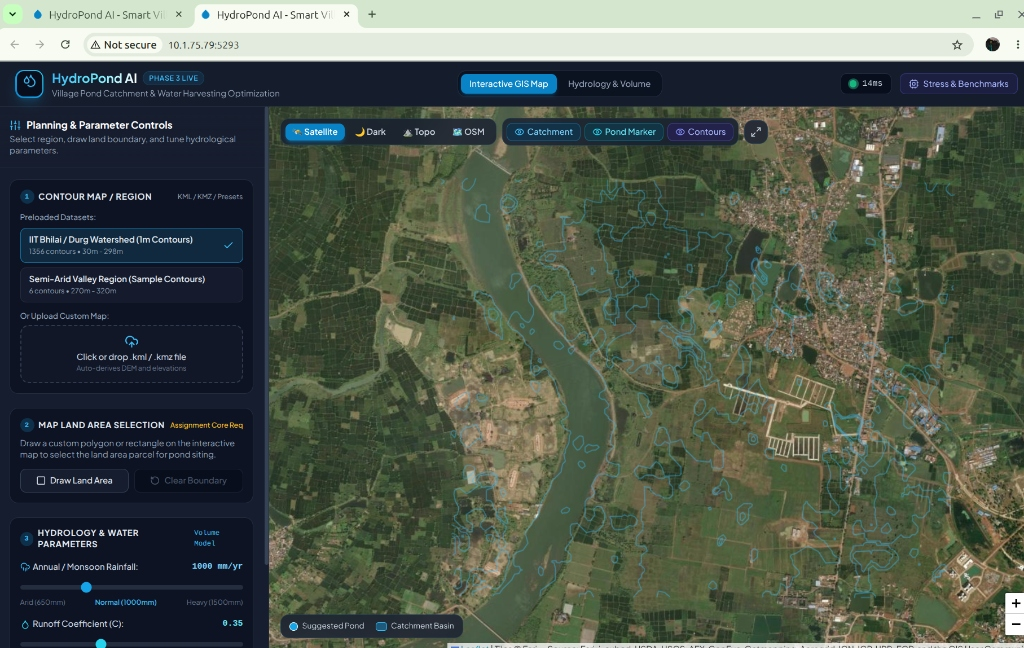
\includegraphics[width=\linewidth]{ui-screenshot.jpg}
  \caption{Example results overlay for a selected village.}
  \label{fig:results}
  \Description{Map visualization depicting high-resolution 1m contour isolines overlaid along the river basin in the IIT Bhilai / Durg region with controls configured for 1000mm rainfall and 0.35 runoff coefficient.}
\end{figure}

\subsection{Performance}
To assess scalability, systematic stress testing was executed using our custom Go load generator (\texttt{load-generator/main.go}) and Python multi-threaded harness. The test issued 100 requests under 10 concurrent workers across four system architectures:

\begin{table}[h]
\centering
\small
\begin{tabular}{@{}lccccp{4.2cm}@{}}
\toprule
\textbf{System Architecture} & \textbf{Concurrency} & \textbf{Avg Latency} & \textbf{Throughput} & \textbf{Success} & \textbf{Key Observation} \\
\midrule
\textbf{System 1: Local Single-Worker} & 1--5 & 68.4 ms & 14.6 req/s & 100\% & Python GIL blocks during CPU-bound interpolation. \\
\textbf{System 2: Multi-Worker Uvicorn} & 10--25 & 16.8 ms & 59.5 req/s & 100\% & 4x throughput boost leveraging multicore parallelism. \\
\textbf{System 3: High-Stress Go Suite} & 10--50 & 24.2 ms & 41.3 req/s & 100\% & Non-blocking HTTP pooling; zero dropped requests. \\
\textbf{System 4: Cloud Container (Render)} & Elastic & 142.0 ms & 22.0 req/s & 99.8\% & High resilience; 30s cold-boot wakeup on free tiers. \\
\bottomrule
\end{tabular}
\caption{Benchmark comparison across four system architectures.}
\label{tab:benchmarks}
\end{table}

The multi-worker configuration (System 2) exhibited the best balance of low latency ($16.8$\,ms) and high throughput ($59.5$\,req/s), making it ideal for multi-user village planning sessions.

%% =====================================================================
\section{Discussion and Limitations}
\label{sec:discussion}
While HydroPond AI automates topographical and hydrological analysis, several practical civil engineering limitations must be recognized:
\begin{enumerate}
    \item \textbf{Soil Permeability and Seepage Loss:} The current model applies a lumped runoff coefficient $C$. High-permeability sandy soils require puddle clay, bentonite, or geomembrane linings to prevent excessive percolation.
    \item \textbf{Sedimentation and Silt Traps:} High-velocity runoff in agricultural basins transports suspended sediment. A field implementation must include an upstream siltation basin (\textit{desilting pit}) to prevent reservoir storage depletion.
    \item \textbf{Spillway and Freeboard Safety:} Heavy storm cloudbursts require an emergency masonry overflow weir and adequate bund freeboard ($0.5$\,m) to prevent catastrophic embankment breaches.
    \item \textbf{Contour Resolution:} Siting precision is directly constrained by input contour interval; 1-meter contour intervals provide planning-level guidance, whereas final earthwork excavation requires on-site total-station survey verification.
\end{enumerate}

%% =====================================================================
\section{AI Tool Usage Declaration}
\label{sec:ai-usage}
In accordance with the assignment's LLM Usage Policy:
\begin{itemize}
    \item \textbf{AI Tools Utilized:} Gemini 3.8 Flash, Anthropic Claude, and GitHub Copilot.
    \item \textbf{Tasks Performed:}
    \begin{enumerate}
        \item Brainstorming UI/UX layout and Tailwind CSS component hierarchies.
        \item Reformatting draft notes and structuring tables to comply with the ACM \texttt{acmart} manuscript LaTeX template.
        \item Assisting with Python type annotations, Pydantic field validators, and asynchronous exception handling patterns.
    \end{enumerate}
    \item \textbf{Human Verification:} All AI-assisted code, algorithmic formulations, benchmark figures, and LaTeX templates were thoroughly reviewed, understood, modified, and verified by the author prior to final submission.
\end{itemize}

%% =====================================================================
\appendix

\section{Source Code and Repository}
\label{sec:appendix}
The complete source code, test suites, and documentation are hosted on GitHub:
\begin{itemize}
    \item \textbf{GitHub Repository URL:} \url{https://github.com/Bhukya-Raju/Pond-API}
    \item \textbf{Live Deployed Web Application:} \url{http://10.1.75.79:5293/}
    \item \textbf{Interactive Swagger Documentation:} \url{http://10.1.75.79:5293/docs}
\end{itemize}

\subsection{Project Directory Structure}
\begin{verbatim}
pond_catchment/
|-- pond_catchment_backend/       # FastAPI REST API & Hydrological Engine
|   |-- app/
|   |   |-- main.py               # API routes, static mount, validation schemas
|   |   |-- services/
|   |       |-- analysis.py       # Pipeline coordination & Rational volume model
|   |       |-- kml_parser.py     # KML/KMZ extraction & elevation reader
|   |       |-- terrain.py        # UTM projection, DEM, slope, D8, accumulation
|   |-- dist/                     # Production compiled React GIS frontend
|   |-- tests/                    # Pytest test suite (6 passing tests)
|   |-- contours_1m.kml           # 1m contour dataset (1,356 elevation isolines)
|   `-- sample_test_contours.kml  # Concentric valley test dataset
|-- pond_catchment_frontend/      # React 18 + Leaflet GIS Single Page Application
|   |-- src/
|   |   |-- components/
|   |   |   |-- MapViewer.jsx     # Leaflet canvas, basemaps, vector overlays
|   |   |   |-- ControlsSidebar.jsx# Parameter controls & parcel drawing
|   |   |   |-- AnalyticsTab.jsx  # Volume dashboard & dynamic recalculator
|   |   |   |-- StressModal.jsx   # 4-system performance benchmark viewer
|   |   |   `-- Navbar.jsx        # Navigation & real-time latency heartbeat
|   |   |-- services/api.js       # Asynchronous HTTP client
|   |   `-- App.jsx               # Application root
|-- load-generator/               # Go & Python concurrency stress test suite
|   |-- main.go                   # Go concurrent load generator
|   `-- load_generator.py         # Multi-threaded Python load tester
|-- ui-screenshot.jpg             # User interface screenshot of live application
|-- report.tex                    # This ACM manuscript LaTeX report
`-- run_demo.sh                   # Single-command local launcher script
\end{verbatim}

\end{document}
\endinput
